\begin{frame}[shrink=35]
%\begin{frame}
  \frametitle{The FEniCS challenge!}
  \begin{columns}[c]
    \begin{column}{0.5\textwidth}
      \begin{itemize}
        \item Domain: \vspace{-1em}
          \begin{align*}
            \Omega_{_{DO}} &= \text{dolphin domain} \\
                    \Omega &= [0,1]\times[0,1] \setminus \Omega_{_{DO}} \\
                    \Omega_1 &= \{ T \in \mesh : T \subset
          B_{0.35}(0.5,0.5) \} \\
            \Omega_2 &= \Omega \setminus \Omega_1 \\
            \partial \Omega_D &= \{0\} \times [0,1] \cup \{1\} \times
            [0,1]
            \\
            \partial \Omega_{N,1} &= \partial \Omega_{_{DO}} \\
            \partial \Omega_{N,2} &= [0,1] \times \{0\} \cup
            [0,1] \times \{1\}               
          \end{align*}
        \item  Conductivity, source and boundary values: 
          \vspace{-0.5em}
          \begin{align*}
            k(x,y) &= 
            \begin{cases}
              10 &\quad \text{in } \Omega_1  \\ 
      50 + e^{50(0.5 - y )^2} &\quad \text{in } \Omega_2
            \end{cases}
            \\
            f(x,y) &= 1
            \\
            g_D(x,y) &= 0 \\
        g_{N,1}(x,y) &= 0 \\
        g_{N,2}(x,y) &= \sin(\pi x)\sin(\pi y)
          \end{align*}
        \item As an alternative, reuse the source function and the
          Dirichlet boundary values from exercise 3:
          \begin{align*}
            f(x,y) &= 2\cos(2\pi x)\cos(2\pi y) 
            \\
            g_D(x,y) &= 0.5 \cos(2\pi y) \quad \text{on } x = 0 \\
            g_D(x,y) &= 1 \quad \text{on } x = 1 \\
          \end{align*}
      \end{itemize}
    \end{column}
    \begin{column}{0.5\textwidth}
      \begin{center}
        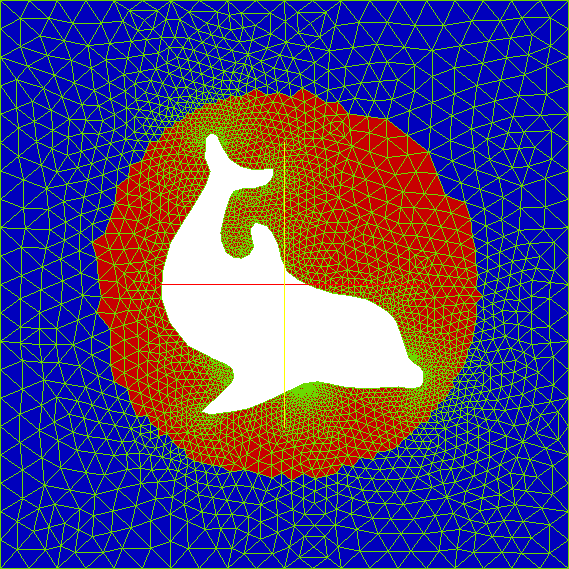
\includegraphics[width=1.0\textwidth]{png/poisson_5_subdomains.png}
      \end{center}
    \end{column}
  \end{columns}
\end{frame}

